*\documentclass{ximera}

%\usepackage{todonotes}

\newcommand{\todo}{}

\usepackage{esint} % for \oiint
\ifxake%%https://math.meta.stackexchange.com/questions/9973/how-do-you-render-a-closed-surface-double-integral
\renewcommand{\oiint}{{\large\bigcirc}\kern-1.56em\iint}
\fi


\graphicspath{
  {./}
  {ximeraTutorial/}
  {basicPhilosophy/}
  {functionsOfSeveralVariables/}
  {normalVectors/}
  {lagrangeMultipliers/}
  {vectorFields/}
  {greensTheorem/}
  {shapeOfThingsToCome/}
  {dotProducts/}
  {partialDerivativesAndTheGradientVector/}
  {../productAndQuotientRules/exercises/}
  {../normalVectors/exercisesParametricPlots/}
  {../continuityOfFunctionsOfSeveralVariables/exercises/}
  {../partialDerivativesAndTheGradientVector/exercises/}
  {../directionalDerivativeAndChainRule/exercises/}
  {../commonCoordinates/exercisesCylindricalCoordinates/}
  {../commonCoordinates/exercisesSphericalCoordinates/}
  {../greensTheorem/exercisesCurlAndLineIntegrals/}
  {../greensTheorem/exercisesDivergenceAndLineIntegrals/}
  {../shapeOfThingsToCome/exercisesDivergenceTheorem/}
  {../greensTheorem/}
  {../shapeOfThingsToCome/}
  {../separableDifferentialEquations/exercises/}
  {vectorFields/}
}

\newcommand{\mooculus}{\textsf{\textbf{MOOC}\textnormal{\textsf{ULUS}}}}

\usepackage{tkz-euclide}
\usepackage{tikz}
\usepackage{tikz-cd}
\usetikzlibrary{arrows}
\tikzset{>=stealth,commutative diagrams/.cd,
  arrow style=tikz,diagrams={>=stealth}} %% cool arrow head
\tikzset{shorten <>/.style={ shorten >=#1, shorten <=#1 } } %% allows shorter vectors

\usetikzlibrary{backgrounds} %% for boxes around graphs
\usetikzlibrary{shapes,positioning}  %% Clouds and stars
\usetikzlibrary{matrix} %% for matrix
\usepgfplotslibrary{polar} %% for polar plots
\usepgfplotslibrary{fillbetween} %% to shade area between curves in TikZ
%\usetkzobj{all}
\usepackage[makeroom]{cancel} %% for strike outs
%\usepackage{mathtools} %% for pretty underbrace % Breaks Ximera
%\usepackage{multicol}
\usepackage{pgffor} %% required for integral for loops



%% http://tex.stackexchange.com/questions/66490/drawing-a-tikz-arc-specifying-the-center
%% Draws beach ball
\tikzset{pics/carc/.style args={#1:#2:#3}{code={\draw[pic actions] (#1:#3) arc(#1:#2:#3);}}}



\usepackage{array}
\setlength{\extrarowheight}{+.1cm}
\newdimen\digitwidth
\settowidth\digitwidth{9}
\def\divrule#1#2{
\noalign{\moveright#1\digitwidth
\vbox{\hrule width#2\digitwidth}}}




% \newcommand{\RR}{\mathbb R}
% \newcommand{\R}{\mathbb R}
% \newcommand{\N}{\mathbb N}
% \newcommand{\Z}{\mathbb Z}

\newcommand{\sagemath}{\textsf{SageMath}}


%\renewcommand{\d}{\,d\!}
%\renewcommand{\d}{\mathop{}\!d}
%\newcommand{\dd}[2][]{\frac{\d #1}{\d #2}}
%\newcommand{\pp}[2][]{\frac{\partial #1}{\partial #2}}
% \renewcommand{\l}{\ell}
%\newcommand{\ddx}{\frac{d}{\d x}}

% \newcommand{\zeroOverZero}{\ensuremath{\boldsymbol{\tfrac{0}{0}}}}
%\newcommand{\inftyOverInfty}{\ensuremath{\boldsymbol{\tfrac{\infty}{\infty}}}}
%\newcommand{\zeroOverInfty}{\ensuremath{\boldsymbol{\tfrac{0}{\infty}}}}
%\newcommand{\zeroTimesInfty}{\ensuremath{\small\boldsymbol{0\cdot \infty}}}
%\newcommand{\inftyMinusInfty}{\ensuremath{\small\boldsymbol{\infty - \infty}}}
%\newcommand{\oneToInfty}{\ensuremath{\boldsymbol{1^\infty}}}
%\newcommand{\zeroToZero}{\ensuremath{\boldsymbol{0^0}}}
%\newcommand{\inftyToZero}{\ensuremath{\boldsymbol{\infty^0}}}



% \newcommand{\numOverZero}{\ensuremath{\boldsymbol{\tfrac{\#}{0}}}}
% \newcommand{\dfn}{\textbf}
% \newcommand{\unit}{\,\mathrm}
% \newcommand{\unit}{\mathop{}\!\mathrm}
% \newcommand{\eval}[1]{\bigg[ #1 \bigg]}
% \newcommand{\seq}[1]{\left( #1 \right)}
% \renewcommand{\epsilon}{\varepsilon}
% \renewcommand{\phi}{\varphi}


% \renewcommand{\iff}{\Leftrightarrow}

% \DeclareMathOperator{\arccot}{arccot}
% \DeclareMathOperator{\arcsec}{arcsec}
% \DeclareMathOperator{\arccsc}{arccsc}
% \DeclareMathOperator{\si}{Si}
% \DeclareMathOperator{\scal}{scal}
% \DeclareMathOperator{\sign}{sign}


%% \newcommand{\tightoverset}[2]{% for arrow vec
%%   \mathop{#2}\limits^{\vbox to -.5ex{\kern-0.75ex\hbox{$#1$}\vss}}}
% \newcommand{\arrowvec}[1]{{\overset{\rightharpoonup}{#1}}}
% \renewcommand{\vec}[1]{\arrowvec{\mathbf{#1}}}
% \renewcommand{\vec}[1]{{\overset{\boldsymbol{\rightharpoonup}}{\mathbf{#1}}}}

% \newcommand{\point}[1]{\left(#1\right)} %this allows \vector{ to be changed to \vector{ with a quick find and replace
% \newcommand{\pt}[1]{\mathbf{#1}} %this allows \vec{ to be changed to \vec{ with a quick find and replace
% \newcommand{\Lim}[2]{\lim_{\point{#1} \to \point{#2}}} %Bart, I changed this to point since I want to use it.  It runs through both of the exercise and exerciseE files in limits section, which is why it was in each document to start with.

% \DeclareMathOperator{\proj}{\mathbf{proj}}
% \newcommand{\veci}{{\boldsymbol{\hat{\imath}}}}
% \newcommand{\vecj}{{\boldsymbol{\hat{\jmath}}}}
% \newcommand{\veck}{{\boldsymbol{\hat{k}}}}
% \newcommand{\vecl}{\vec{\boldsymbol{\l}}}
% \newcommand{\uvec}[1]{\mathbf{\hat{#1}}}
% \newcommand{\utan}{\mathbf{\hat{t}}}
% \newcommand{\unormal}{\mathbf{\hat{n}}}
% \newcommand{\ubinormal}{\mathbf{\hat{b}}}

% \newcommand{\dotp}{\bullet}
% \newcommand{\cross}{\boldsymbol\times}
% \newcommand{\grad}{\boldsymbol\nabla}
% \newcommand{\divergence}{\grad\dotp}
% \newcommand{\curl}{\grad\cross}
%\DeclareMathOperator{\divergence}{divergence}
%\DeclareMathOperator{\curl}[1]{\grad\cross #1}
% \newcommand{\lto}{\mathop{\longrightarrow\,}\limits}

% \renewcommand{\bar}{\overline}

\colorlet{textColor}{black}
\colorlet{background}{white}
\colorlet{penColor}{blue!50!black} % Color of a curve in a plot
\colorlet{penColor2}{red!50!black}% Color of a curve in a plot
\colorlet{penColor3}{red!50!blue} % Color of a curve in a plot
\colorlet{penColor4}{green!50!black} % Color of a curve in a plot
\colorlet{penColor5}{orange!80!black} % Color of a curve in a plot
\colorlet{penColor6}{yellow!70!black} % Color of a curve in a plot
\colorlet{fill1}{penColor!20} % Color of fill in a plot
\colorlet{fill2}{penColor2!20} % Color of fill in a plot
\colorlet{fillp}{fill1} % Color of positive area
\colorlet{filln}{penColor2!20} % Color of negative area
\colorlet{fill3}{penColor3!20} % Fill
\colorlet{fill4}{penColor4!20} % Fill
\colorlet{fill5}{penColor5!20} % Fill
\colorlet{gridColor}{gray!50} % Color of grid in a plot

\newcommand{\surfaceColor}{violet}
\newcommand{\surfaceColorTwo}{redyellow}
\newcommand{\sliceColor}{greenyellow}




\pgfmathdeclarefunction{gauss}{2}{% gives gaussian
  \pgfmathparse{1/(#2*sqrt(2*pi))*exp(-((x-#1)^2)/(2*#2^2))}%
}


%%%%%%%%%%%%%
%% Vectors
%%%%%%%%%%%%%

%% Simple horiz vectors
\renewcommand{\vector}[1]{\left\langle #1\right\rangle}


%% %% Complex Horiz Vectors with angle brackets
%% \makeatletter
%% \renewcommand{\vector}[2][ , ]{\left\langle%
%%   \def\nextitem{\def\nextitem{#1}}%
%%   \@for \el:=#2\do{\nextitem\el}\right\rangle%
%% }
%% \makeatother

%% %% Vertical Vectors
%% \def\vector#1{\begin{bmatrix}\vecListA#1,,\end{bmatrix}}
%% \def\vecListA#1,{\if,#1,\else #1\cr \expandafter \vecListA \fi}

%%%%%%%%%%%%%
%% End of vectors
%%%%%%%%%%%%%

%\newcommand{\fullwidth}{}
%\newcommand{\normalwidth}{}



%% makes a snazzy t-chart for evaluating functions
%\newenvironment{tchart}{\rowcolors{2}{}{background!90!textColor}\array}{\endarray}

%%This is to help with formatting on future title pages.
\newenvironment{sectionOutcomes}{}{}



%% Flowchart stuff
%\tikzstyle{startstop} = [rectangle, rounded corners, minimum width=3cm, minimum height=1cm,text centered, draw=black]
%\tikzstyle{question} = [rectangle, minimum width=3cm, minimum height=1cm, text centered, draw=black]
%\tikzstyle{decision} = [trapezium, trapezium left angle=70, trapezium right angle=110, minimum width=3cm, minimum height=1cm, text centered, draw=black]
%\tikzstyle{question} = [rectangle, rounded corners, minimum width=3cm, minimum height=1cm,text centered, draw=black]
%\tikzstyle{process} = [rectangle, minimum width=3cm, minimum height=1cm, text centered, draw=black]
%\tikzstyle{decision} = [trapezium, trapezium left angle=70, trapezium right angle=110, minimum width=3cm, minimum height=1cm, text centered, draw=black]


\title{Open Sets}

\begin{document}

\begin{abstract}
always room
\end{abstract}
\maketitle





Why do we call $(1, 5)$ an \textbf{open interval} on the real line or in the real numbers? \\



The reason is that each number in the interval feels like it is out in the open - that there is room around it.  It may be a very small surrounding space around it, but room none-the-less.  


We extend this idea that there is always room ``around'' each number to \textbf{open sets in $\mathbb{R}$}.






\section*{Open Sets in $\mathbb{R}$}

In an open set in $\mathbb{R}$, each number has room on either side.  




\begin{definition}  \textbf{\textcolor{green!50!black}{Open Set in $\mathbb{R}$}}


$S \subset \mathbb{R}$ is an \textbf{open set in $\mathbb{R}$} provided 

\[
\text{For each } a \in S, \text{ there exists an } \epsilon > 0 \text{ such that }  (a - \epsilon, a + \epsilon) \subset S
\]

\end{definition}



\begin{idea}

The idea is that inside an open set, every number sits inside an open interval inside the set.  There is space between each number and the endpoint. There is a positive distance between each number and each endpoint.
\end{idea}

Forcing a positive distance between each number and the endpoints turns out to have far reaching consequences, which we will investigate in this course.  First, we need some language for open sets. \\



\begin{example}  \textit{Open Intervals in $\mathbb{R}$}


The open interval $(4,7)$ is an open set in $\mathbb{R}$.


\begin{image}
  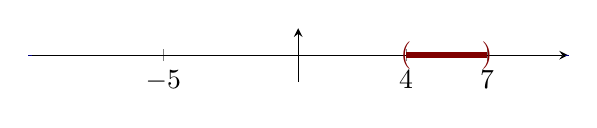
\begin{tikzpicture}
  \begin{axis}[
            %xmin=-25,xmax=25,ymin=-25,ymax=25,
            %width=3in,
            clip=false,
            axis lines=center,
            %ticks=none,
            unit vector ratio*=1 1 1,
            ymajorticks=false,
            xtick={-5,4, 7},
            %xlabel=$x$, ylabel=$y$,
            %every axis y label/.style={at=(current axis.above origin),anchor=south},
            every axis x label/.style={at=(current axis.right of origin),anchor=west},
          ]      
       
            \addplot [line width=2, penColor2, smooth,samples=100,domain=(4:7)] ({x},{0});

            \addplot [line width=0.5, penColor, smooth,samples=100,domain=(-10:-9.9)] ({x},{0});
            \addplot [line width=0.5, penColor, smooth,samples=100,domain=(9.9:10)] ({x},{0});


            \node at (axis cs:4,0) [penColor2] {$($};
            \node at (axis cs:7,0) [penColor2] {$)$};

    \end{axis}
  \end{tikzpicture}
  \end{image}







\begin{image}
  \begin{tikzpicture}
  \begin{axis}[
            %xmin=-25,xmax=25,ymin=-25,ymax=25,
            %width=3in,
            clip=false,
            axis lines=center,
            %ticks=none,
            unit vector ratio*=1 1 1,
            ymajorticks=false,
            xtick={-5,4, 7},
            %xlabel=$x$, ylabel=$y$,
            %every axis y label/.style={at=(current axis.above origin),anchor=south},
            every axis x label/.style={at=(current axis.right of origin),anchor=west},
          ]      
       
            \addplot [line width=2, penColor2, smooth,samples=100,domain=(4:7)] ({x},{0});

            \addplot [line width=0.5, penColor, smooth,samples=100,domain=(-10:-9.9)] ({x},{0});
            \addplot [line width=0.5, penColor, smooth,samples=100,domain=(9.9:10)] ({x},{0});

            \addplot [color=penColor2, fill=white,only marks,mark=*] coordinates{(4,0)};
            \addplot [color=penColor2, fill=white,only marks,mark=*] coordinates{(7,0)};


    \end{axis}
  \end{tikzpicture}
  \end{image}




\begin{explanation}

Let $c$ be any number in $(4,7)$.  Then the open subinterval $\left( c - \frac{4+c}{2}, c + \frac{7+c}{2} \right)$ will always be inside $(4,7)$.

Therefore, for each $c \in (4, 7)$, there exists an open interval inside $(4,7)$, which contains $c$.

Since this is true for all of the numbers in $(4,7)$, the interval is an open set in $\mathbb{R}$.

\end{explanation}
\end{example}









\begin{example}  



The interval $(4,7]$ is not an open set in $\mathbb{R}$.


\begin{image}
  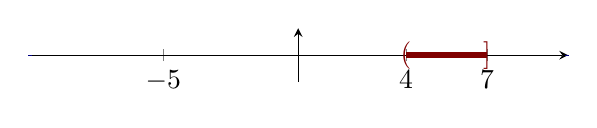
\begin{tikzpicture}
  \begin{axis}[
            %xmin=-25,xmax=25,ymin=-25,ymax=25,
            %width=3in,
            clip=false,
            axis lines=center,
            %ticks=none,
            unit vector ratio*=1 1 1,
            ymajorticks=false,
            xtick={-5,4, 7},
            %xlabel=$x$, ylabel=$y$,
            %every axis y label/.style={at=(current axis.above origin),anchor=south},
            every axis x label/.style={at=(current axis.right of origin),anchor=west},
          ]      
       
            \addplot [line width=2, penColor2, smooth,samples=100,domain=(4:7)] ({x},{0});

            \addplot [line width=0.5, penColor, smooth,samples=100,domain=(-10:-9.9)] ({x},{0});
            \addplot [line width=0.5, penColor, smooth,samples=100,domain=(9.9:10)] ({x},{0});


            \node at (axis cs:4,0) [penColor2] {$($};
            \node at (axis cs:7,0) [penColor2] {$]$};

    \end{axis}
  \end{tikzpicture}
  \end{image}








\begin{image}
  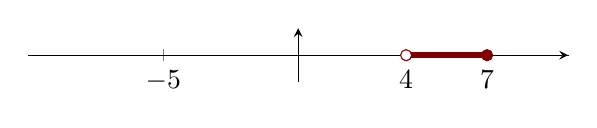
\begin{tikzpicture}
  \begin{axis}[
            %xmin=-25,xmax=25,ymin=-25,ymax=25,
            %width=3in,
            clip=false,
            axis lines=center,
            %ticks=none,
            unit vector ratio*=1 1 1,
            ymajorticks=false,
            xtick={-5,4, 7},
            %xlabel=$x$, ylabel=$y$,
            %every axis y label/.style={at=(current axis.above origin),anchor=south},
            every axis x label/.style={at=(current axis.right of origin),anchor=west},
          ]      
       
            \addplot [line width=2, penColor2, smooth,samples=100,domain=(4:7)] ({x},{0});

            \addplot [line width=0.5, penColor, smooth,samples=100,domain=(-10:-9.9)] ({x},{0});
            \addplot [line width=0.5, penColor, smooth,samples=100,domain=(9.9:10)] ({x},{0});


            \addplot [color=penColor2,only marks,mark=*] coordinates{(7,0)};
            \addplot [color=penColor2, fill=white,only marks,mark=*] coordinates{(4,0)};


    \end{axis}
  \end{tikzpicture}
  \end{image}






\begin{explanation}

Consider the number $7$.  Any open interval around $7$ would look like $(7 - \epsilon, 7 + \delta)$, with both $\epsilon > 0$  and $\delta > 0$.  However, there is always a real number in the interval $(7, 7 + \delta)$, like $7 + \frac{\delta}{2}$, which lies outside $(4, 7]$.

Therefore, no matter which open interval you choose around $7$, it will always containing a number outside $(4, 7]$.

$(4, 7]$  is not an open set in $\mathbb{R}$.

\end{explanation}
\end{example}

$\blacktriangleright$ Open intervals cannot contain their endpoints. \\





\begin{example}  \textit{Unions of Open Intervals} \\


Any union of open intervals is itself an open set.



\begin{explanation}

Let $S$ be a union of open intervals.  \\
Let $c \in S$. \\
Then $c$ is in one of the open intervals. \\
Then there exists an $\epsilon > 0$, such that $(c - \epsilon, c + \epsilon)$ is a subset of this one open interval.  This interval is a subset of $S$.  Therefore, $(c - \epsilon, c + \epsilon) \subset S$. \\


\end{explanation}

\end{example}















\begin{example}  \textit{The Empty Set} \\


The \textbf{empty set}, $\emptyset$, is the set with no element.  The empty set is a subset of the real numbers.  It is the subset containing no real numbers. \\


$\emptyset$ is an open set. \\



\begin{explanation}


The reasoning is sort of reverse thinking.  If $\emptyset$ is not open, then it MUST contain a number, such that there is no tiny open interval around it.  There is no such number.  Therefore, $\emptyset$ is an open set.


\end{explanation}

\end{example}

$\blacktriangleright$ These types of statements are often said to be \textbf{vacuously true}.  They are true, because there is nothing that violates the definition - because there isn't anything at all. 











\begin{center}
\textbf{\textcolor{green!50!black}{ooooo-=-=-=-ooOoo-=-=-=-ooooo}} \\

more examples can be found by following this link\\ \link[More Examples of Real-Valued Functions]{https://ximera.osu.edu/csccmathematics/precalculus1/precalculus1/realValued/examples/exampleList}

\end{center}



\end{document}
